\section{Forschungsstand}\raggedbottom 
Karten in Videobildern zu erkennen stellt ein Problem der Objekterkennung dar.
Eine häufig verwendete Methode zur Objekterkennung sind Bildmerkmale.
Im Folgenden werden die Konzepte der Merkmalsdetektion (Feature Detection), Merkmalsbeschreibung (Feature Description) und des Merkmalsabgleiches (Feature Matching) beschrieben.
Desweiteren werden grundlegende Verfahren und Methoden der digitalen Bildverarbeitung erläutert, die in dieser Arbeit wichtig sind.

\subsection{Digitale Bildverarbeitung}

\subsubsection{Bildbeschreibung}

In der digitalen Bildverarbeitung gibt es mehrere Möglichkeiten, ein Bild zu beschreiben. Zwei häufig genutzte Bildbeschreibungen sind Rasterbilder und Vektorgrafiken \footnote{\cite[S. 15]{Burg06}}. In dieser Arbeit werden ausschließlich Rasterbilder betrachtet.

Ein Rasterbild ist eine zweidimensionale Matrix $I$ der Größe $n \times m$. Diese Größe wird im weiterem Auflösung genannt. Jedes Element dieser Matrix wird als Pixel bezeichnet.
Welche Informationen in jedem Pixel gespeichert sind, hängt von dem Typ des Bildes ab. Für diese Arbeit wichtig sind Grauwertbilder und Farbbilder.

Grauwertbilder speichern für jeden Pixel einen Wert zwischen 0 und 255. Dieser Wert beschreibt die Helligkeit bzw. Intensität an diesem Bildpunkt. Ein Wert von 0 steht hierbei für keine Helligkeit und ist somit schwarz. Ein Wert von 255 stellt eine maximale Helligkeit dar und ist somit weiß. 

Farbbilder speichern in jedem Pixel drei Komponenten für die drei Primärfarben Rot, Grün und Blau. Die Werte für die einzelnen Komponenten liegen jeweils zwischen 0 bis 255. Die einzelnen Komponenten kodieren, wie bei Graubildern, die Intensität der jeweiligen Farbe an dem Pixel.

\subsubsection{Umwandlung von Farb- zu Graubild}

Bilder müssen für verschiedene Anwendungen von einem Farbbild in ein Graubild umgewandelt werden. Dabei soll die Helligkeit einer Farbe übernommen werden, während die Farbinformationen verloren gehen.

Bei der Umwandlung wird jeder Pixel einzeln von einem Farbwert in einen Grauwert überführt.
Dabei trägt jede der Primärfarben einen unterschiedlichen Teil zur Helligkeit eines Pixels bei.
Seien R, G und B jeweils die Werte der einzelnen Farbkomponenten für den betrachteten Pixel.
Die Formel für den Grauwert eines Pixels ist nach der Empfehlung BT.601\footnote{\cite[S. 3]{international2007studio}} der International Telecommunications Union:

\[
0.299R +  0.587G + 0.144B
\] 

Es sei angemerkt, dass es noch weitere Verfahren zur Umwandlung von Farbbilder zu Graubildern gibt \footnote{\cite[S. 4]{international2002parameter}}.

\subsubsection{Kontrast}
\label{sec:kontrast}

Der Kontrast eines Bildes oder eines Bildausschnittes beschreibt das Verhältnis der maximalen zur minimalen Helligkeit bzw. Intensität. Ein Bild mit einem hohen Kontrast hat eine große Differenz zwischen der maximalen und minimalen Helligkeit.

\subsubsection{Bildrauschen}
\label{sec:rauschen}

Bei digitalen Bildern, die mit einer Kamera aufgenommen wurden, treten häufig kleine Störungen im Bild auf. Dadurch enstehen Pixel, die von der eigentlichen Farbe oder Helligkeit des Bildes abweichen. Diese Störungen im Bild werden als Bildrauschen bezeichnet. 


\subsubsection{Filter}

In der Bildverarbeitung stellen Filter eine Möglichkeit dar, verschiedene Operationen auf einem Bild auszuführen. So können Filter z.B. genutzt werden, um ein Bild zu glätten oder zu schärfen \footnote{\cite[S. 99f]{Burg06}}. Im Folgenden werden nur lineare Filter betrachtet.

Ein Filter berechnet für ein gegebenes Bild neue Werte für alle Pixel oder auch nur einer Auswahl an Pixeln. Hierbei hängt der Wert nicht nur von dem ursprünglichen Wert des Pixels ab, sondern i.d.R auch von den Werten der anderen Pixeln in der Umgebung. Diese Umgebung wird auch Filterregion genannt. Diese Regionen sind i.d.R quadratisch.
Wie sehr die einzelnen Pixel in der Region in den neuen Wert einfließen, bestimmt eine Filtermatrix. Diese Matrix wird mit ihrem Mittelpunkt über den zu verändernen Pixel gelegt. Es werden alle Pixelwerte mit dem jeweils überlappenden Matrixwert multipliziert und aufaddiert. Das Ergebnis ist der neue Pixelwert (siehe Abbildung \ref{fig:filter}). 

Für eine $3 \times 3$ große Filterregion mit der Filtermatrix $H(i, j) \in \mathbb{R}^{3 \times 3}$ kann der neue Pixelwert $I'(u, v)$ für den Punkt $(u, v)$ wie folgt berechnet werden

\[
I'(u, v) = \sum_{i = -1}^1 \sum_{j = -1}^1  I(u + i, v + j) H(i, j)
\]


\begin{figure}[h]
    \centering
		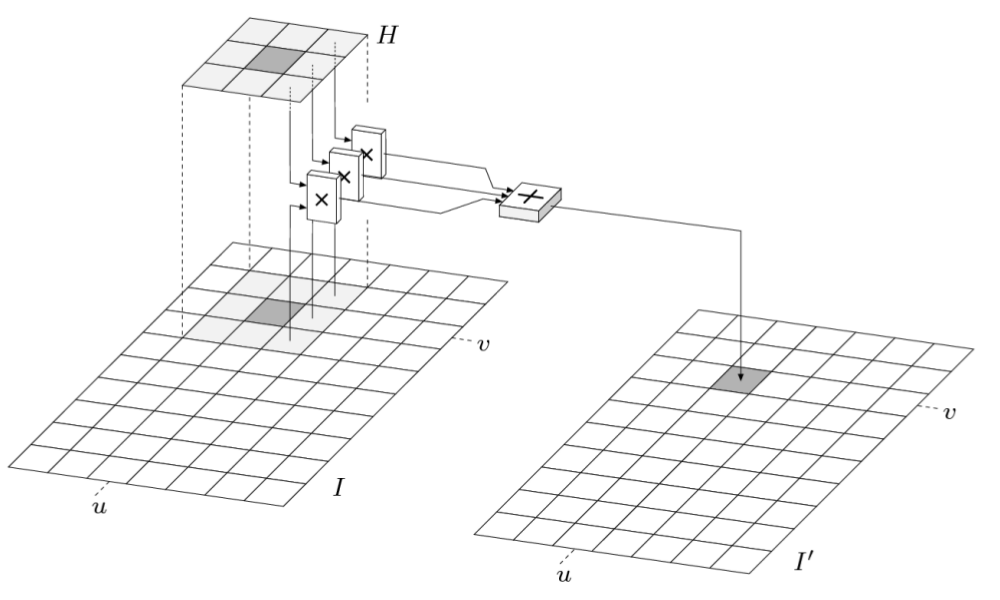
\includegraphics[scale=0.35]{bilder/filter.png}
    	\caption{Darstellung der Filteroperation für ein Bild I und die Filtermatrix H. (Abbildung aus \cite[S. 92]{Burg06})}
    	\label{fig:filter}
\end{figure}

\subsubsection{Gaußfilter}

Der Gaußfilter ist ein Glättungsfilter, bei dem die Werte der Filtermatrix einer diskreten zweidimensionalen Gaußfunktion entsprechnen.

\[
G(x, y, \sigma) = \frac{1}{2\pi\sigma^2} e^{-\frac{(x^2 + y^2)}{2 \sigma^2}}
\]

Je weiter ein Pixel vom betrachteten Punkt entfernt ist, umso geringer ist sein Einfluss auf das Filterergebnis.
Wie stark diese Werte abnehmen lässt sich mit der Standardabweichung $\sigma$ kontrollieren.

\subsubsection{Douglas-Peucker-Algorithmus}
\label{sec:douglas}

Der Douglas-Peucker-Algorithmus ist ein Algorithmus, der einen Streckenzug von Punkten durch weglassen einzelner Punkte approximiert \footnote{\cite{douglasalgorithms}}.
Der Algorithmus startet mit der direkten Verbindung der Endpunkte und fügt rekursiv Zwischenpunkte hinzu, bis eine ausreichend gute Approximation gefunden wurde.

Sei $K = (P_1, P_2, ..., P_n)$ der gegebene Streckenzug mit n Punkten. Zudem wird eine Toleranz $\epsilon$ gewählt.

K wird durch die Strecke $\overline{P_1P_n}$ approximiert. Nun wird geprüft, ob diese Approximation ausreichend ist.
Hierfür werden die inneren Punkte zwischen $P_1$ und $P_n$ betrachtet.

Es wird der innere Punkt $P_m$ mit dem größten Abstand $d_{max}$ zur Strecke $\overline{P_1P_n}$ gesucht.
Die Approximation ist ausreichend, wenn es keine inneren Punkte gibt oder $d_{max} \leq \epsilon$ ist. Wird die Approximation als ausreichend befunden, werden alle inneren Punkte verworfen. Ist die Approximation nicht ausreichen, wird der Streckenzug $K$ in zwei Teilfolgen $K_1 = (P_1, ..., P_m)$ und $K_2 = (P_m, ... , P_n)$ aufgeteilt. Diese beiden Teilfolgen werden nun mit dem gleichen Algorithmus approximiert.

Das Endergebnis besteht aus allen Punkten, die nicht verworfen wurden. Keiner der verworfenen Punkte hat zu dem so enstehenden Streckenzug einen größeren Abstand als $\epsilon$.


\subsubsection{Haar Merkmal}
\label{sec:haar}

Ein Haar Merkmal (Haar-like features) beschreibt den Helligkeitsunterschied von zwei aneinanderliegenden rechteckigen Regionen in einem Bild \footnote{\cite{Viola01rapidobject}}.
Für beide Regionen wird die Summe der Intensität aller Pixel berechnet. Diese beiden Summen werden von einander substrahiert. Der so enstehende Wert für den Helligkeitsunterschied bildet das Haar Merkmal.

Die Wahl der Regionen bestimmt, welche Bildeigenschaften das Merkmal darstellt. Die in Abbildung \ref{fig:haar} dargestellten Regionen sind geeignet, um horizontale bzw. vertikale Kanten zu erkennen.


\begin{figure}[h]
    \centering
		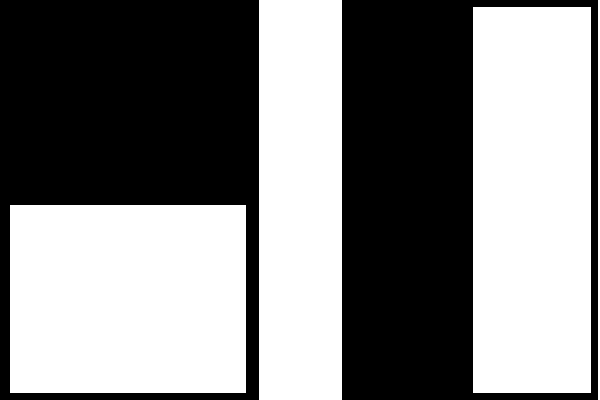
\includegraphics[scale=0.25]{bilder/haar.png}
    	\caption{Beispiel für zwei Haar Merkmale. Der jeweils schwarze und weiße Bereich markiert die Regionen. }
    	\label{fig:haar}
\end{figure}


\subsubsection{Skalenraum}

Ein Objekt, das von einem Menschen beobachtet wird, weist optisch verschiedene Strukturen auf, abhängig von der Distanz zu diesem Objekt. Wird ein Objekt aus großer Entfernung betrachtet, gehen kleinere Strukturen verloren und nur große Strukturen bleiben bestehen.
So lassen sich z.B. aus der Nähe die Blätter eines Baumes betrachten. Aus einer größeren Entfernung hingegen sind die Blätter nicht mehr zu erkennen und nur die grundlegende Form des Baumes.
Der Begriff der Skalierung beschreibt, wie groß dieser Effekt ist. Je höher die Skalierung, um so weniger Details sind erkennerbar.

Der Skalenraum ist ein Konzept der Bildverarbeitung, das ein Bild in verschiedenen Skalierungen darstellen kann \footnote{\cite{Lindeberg94scale-spacetheory:}}. Hierbei kann die Skalierung durch einen kontinuierlichen Skalenparameter $\sigma$ kontrolliert werden.

Um die Skalierung eines Bildes zu erhöhen, wird das Bild geglättet. Durch diese Glättung werden kleine Strukturen unterdrückt (siehe Abbildung \ref{fig:scaleSpace}). Die Glättung wird mit einem Gaußfilter erzeugt \footnote{\cite{Lindeberg94scale-spacetheory:}}. Der Skalenparameter entspricht hierbei der Standardabweichung des Gaußfilters.

Die Skalenraumfunktion eines Bildes wird als $L(x, y, \sigma)$ definiert. Hierbei bestimmt das $\sigma$ die Skalierung. Es gilt mit $*$ als Faltungsoperation für das Bild $I(x, y)$:

\[
L(x, y, \sigma) = G(x, y, \sigma) * I(x, y)
\] 


Wobei $G(x, y, \sigma)$ die 2-Dimensionale Gauß Funktion ist.

\[
G(x, y, \sigma) =  \frac{1}{2 \pi \sigma^{2}} e^{-\frac{(x^2+y^2)}{2\sigma^2}}
\]

Der Skalenraum lässt sich in sogenannte Oktaven einteilen. Eine Oktave im Skalenraum ist jeweils eine Verdoppelung bzw. Halbierung der Skalierung.

\begin{figure}[h]
    \centering
		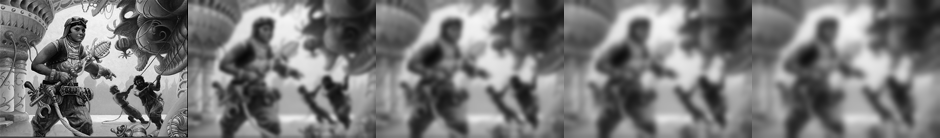
\includegraphics[scale=0.5]{bilder/scaleSpace.png}
    	\caption{Veränderung eines Bildes im Skalenraum. Die Werte für $\sigma$ von links nach rechts: 0, 1.7, 3.4, 5.1, 6.8 und 8.5.}
    	\label{fig:scaleSpace}
\end{figure}


\subsection{Bildmerkmale}

Bildmerkmale stellen eine Möglichkeit dar, bestimmte Punkte oder auch Objekte in einem Bild auf einem anderen Bild wiederzufinden.
Ein einzelnes Merkmal ist eine vektorielle Darstellung eines kleinen Bildbereiches.

Um Merkmale für ein gegebenes Bild zu finden werden zwei Schritte vollzogen.

\begin{itemize}
\item Merkmalsdetektion, findet Punkte im Bild, die sich gut für Merkmale eignen. Diese Punkte werden im Weiteren auch als Keypoints bezeichnet.
\item Merkmalsbeschreibung, wandelt Punkte in eine vektorielle Darstellung um. Im Weiteren auch Deskriptor genannt.
\end{itemize}

Es gibt eine große Anzahl an Methoden, um diese beiden Schritte durchzuführen (siehe Tabelle \ref{table:featureMethods}).
In dieser Arbeit werden die drei Methoden ''Scale-Invariant Feature Transform'' (SIFT), ''Speeded Up Robust Features'' (SURF) und ''Oriented FAST and Rotated BRIEF'' (ORB) betrachtet. 

\begin{table}
\centering
	\begin{tabular}{  l c c   }
	  Methode & Merkmalsdetektion & Merkmalsbeschreibung \\
	  \midrule
	  Harris Corner Detection & X & - \\
	  Features from Accelerated Segment Test & X & - \\
	  Binary Robust Independent Elementary Features & - & X \\
	  Scale-Invariant Feature Transform & X & X \\
	  Speeded-Up Robust Features & X & X \\
	  Oriented FAST and Rotated BRIEF & X & X \\
	  
	\end{tabular}
\caption{Übersicht häufig verwendeter Merkmalsdetektoren und Merkmalsbeschreibern.}
\label{table:featureMethods}
\end{table}

\subsubsection{Merkmalsdetektion}
\label{sec:featureDetection}
Der erste Schritt ist das Finden von Bildausschnitten, die Eigenschaften haben, die möglichst einzigartig sind und sich auch in anderen Bildern wiedererkennen lassen. Diese Merkmale sollen so gewählt werden, dass sie auch nach Rotationen oder Veränderung der Bildgröße bestehen bleiben. Flächen ohne große Veränderungen oder Kanten lassen sich schlecht in Bildern wiederfinden.
Dies lässt sich einfach mit einem Stück blauen Himmel in einem Bild vorstellen. Der Bildausschnitt des Himmels hat keine besonderen Eigenschaften, die ihn einfach von anderen Himmelstücken in Bildern unterscheiden.
Eine Kante hingegen lässt sich deutlich besser wiederfinden. Jedoch ist es bei einem Ausschnitt einer Kante schwer festzustellen, wo sich dieser Ausschnitt entlang der gesamten Kante befindet.
Ecken hingegen sind eindeutiger in einem Bild lokalisierbar.

In Abbildung \ref{fig:featureSample} ist ein Beispiel für die Keypoints, die gefunden werden, zu sehen.

\begin{figure}[h]

    \centering
		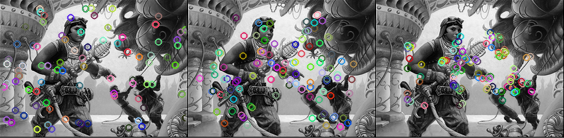
\includegraphics[scale=0.8]{bilder/featureSample.png}
    	\caption{Von links nach rechts die gefundenen Keypoints von SIFT, SURF und ORB. Keypoints sind jeweils mit einem farbigen Kreis markiert. Die Farben haben keine Aussage über den Keypoint und dienen nur der besseren Unterscheidung nahe liegender Punkte. Die Anzahl der gezeigeten Keypoints ist für eine bessere Übersicht jeweils auf 100 beschränkt}
\label{fig:featureSample}
\end{figure}

\subsubsection{Merkmalsdeskription}

Von den Bildausschnitten, die von der Merkmalserkennung als interessant befunden wurden, soll nun in diesem Schritt ein Merkmalsvektor erstellt werden.
Dieser Vektor soll den Ausschnitt so beschrieben, dass für den gleichen Ausschnitt aus einem anderen Bild der Deskriptorvektor sehr ähnlich ist.


\subsubsection{Merkmalsabgleich}

Nachdem die Merkmalsvektoren für interessante Bildausschnitte erstellt wurden, kann nun versucht werden, Merkmale aus einem Bild in einem anderen wiederzufinden.
Da die Vektoren so konstruiert sind, dass ähnliche Bereiche zu ähnlichen Vektoren führen, kann ein Merkmal eines Bildes in einem anderen wiedergefunden werden, indem man den Vektor mit der geringsten Distanz findet.


In Abbildung \ref{fig:matchingSample} ist ein Beispiel für den Merkmalsabgleich zu sehen. Die Merkmale des gedrehten Bildes werden in denen des nicht gedrehten wiedergefunden werden.

\begin{figure}[h]

    \centering
		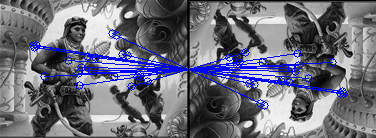
\includegraphics[scale=0.8]{bilder/matchingSample.png}
    	\caption{Die zusammengehörigen Keypoints sind jeweils mit einer Linie verbunden. Die Zahl der gezeigten Matches ist zur besseren Übersicht auf 20 beschränkt.}    	\label{fig:matchingSample}
\end{figure}


\subsubsection{Features from Accelerated Segment Test}
\label{sec:fast}

Das in Edward Rostens und Tom Drummonds Paper ''Machine learning for high-speed corner detection'' \footnote{\cite{Rosten:2006:MLH:2094437.2094478}}  vorgestellte Verfahren ''Features from Accelerated Segment Test'' (FAST) ist ein Merkmalsdetektor.

Damit ein Punkt $p$ mit Intensität $I_p$ als Keypoint erkannt wird, betrachtet FAST einen Kreis um den Punkt. Es wird geprüft, ob es in diesem Kreis eine Menge mit $n$ zusammenhängenden Pixeln gibt, die eine der folgenden Bedingungen erfüllt:

\begin{itemize}
\item Die Intensität jedes Pixels in der Menge ist kleiner als $I_p - t$, wobei t eine konstante Schwelle ist
\item Die Intensität jedes Pixels in der Menge ist größer als $I_p + t$, wobei t eine konstante Schwelle ist
\end{itemize}

Ist eine dieser Bedingunen erfüllt, wird der Punkt als Keypoint erkannt.

\subsection{Weitere Methoden}

\subsubsection{k-nächste-Nachbarn}
\label{sub:knn}

Der k-nächste-Nachbarn (k-Nearest-Neighbors) Algorithmus ist eine Klassifikationsmethode, mit der neue Datenpunkte anhand schon bekannter Daten klassifiziert werden können \footnote{\cite{doi:10.1080/00031305.1992.10475879}}.

Sei $x \in \mathbb{R}^n$ der neue Datenpunkt, der einer von $m \in \mathbb{R}$ verschiedenen Klassen zugeordnet werden soll. Zudem sei $D \subseteq \mathbb{R}^n$ die Menge an Punkten, deren wahre Klasse bekannt ist.

\begin{figure}[h]
    \centering
		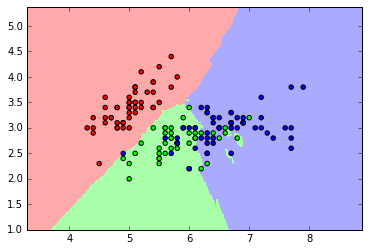
\includegraphics[scale=0.45]{bilder/knn.png}
    	\caption{k-nächste-Nachbarn Klassifikation für drei Klassen (Rot, Blau, Grün). Die Datenpunkte jeder Klasse sind farblich eingezeichnet. Die farbigen Bereiche zeigen an, wie ein neuer Datenpunkt klassifiziert wird, wenn er in diesen liegt.}
    	\label{fig:knn}
\end{figure}

Nun wird ein $k$ gewählt und die $k$ nächsten Nachbarn von x in $D$ gesucht. Nun wird $x$ die Klasse zugewiesen, die durch eine einfache Mehrheitswahl der k nächsten Nachbarn bestimmt wird.
Eine Visualisierung dieser Klassifikation ist in Abbildung \ref{fig:knn} dargestellt.

\subsubsection{Hamming Distanz}
\label{sub:hammingDistanz}

Die Hamming Distanz ist eine Methode, mit der die Ähnlichkeit von zwei gleichlangen Zeichenketten gemessen werden kann \footnote{\cite{hamming}}.
Sie ist definiert als die Anzahl der unterschiedlichen Stellen in den beiden Zeichenketten. 
Die Hamming Distanz kann auch genutzt werden, um die Binärdarstellung zweier Zahlen zu vergleichen. So ist z.B. die Hamming Distanz von $1001$ und $0000$:
\[
H(1001, 0000) = 2
\]


\subsection{Scale-Invariant Feature Transform (SIFT)}
Das folgende Kapitel basiert auf David G. Lowes Paper ''Distinctive Image Features
from Scale-Invariant Keypoints'' \footnote{\cite{Lowe2004}}

In seinem Paper ''Distinctive Image Features from Scale-Invariant Keypoints'' von 2004 stellte David G. Lowe eine Methode zur Merkmalsfindung und Merkmalsbeschreibung vor.

Das Verfahren wurde mit dem Ziel entworfen, dass Merkmale unabhängig von Rotation und Skalierung gefunden werden. So sollen Objekte in Bildern wiedergefunden werden können, wenn sie gedreht oder näher bzw. weiter weg sind.

Die SIFT Merkmale werden in 4 Schritten berechnet.

\begin{enumerate}

\item Extrema im Skalenraum finden, die potentielle Keypoints sein können
\item Prüfen, ob die zuvor gefundenen Punkte geeignete Keypoints sind
\item Zuweisen einer Orientierung für den Bildausschnitt
\item Erstellen des Deskriptors

\end{enumerate}

\subsubsection{Merkmalserkennung}

Da SIFT versucht Merkmale zu finden, die für verschiedene Skalierungen des Bildes konstant sind, müssen Punkte gefunden werden, die invariant zur Skalierung des Bildes sind.
Für die Erkennung von Merkmalen soll sich also nicht auf Details, die in höheren Skalierungen verloren gehen verlassen, sondern Punkte gefunden werden, die im Skalenraum Extrema sind.

Es wurde von Lowe gezeigt \footnote{\cite{Lowe:1999:ORL:850924.851523}}, dass Merkmale im Skalenraum durch Extrema der Differenz der Gauß Funktionen gefunden werden können.
Sei $I(x, y)$ das Bild, $G(x, y, \sigma)$ die zwei Dimensionale Gaußfunktion  und $L(x, y, \sigma)$ die Skalenraumfunktion.
Die Differenz der Gaußfunktionen $D(x, y, \sigma)$ für zwei Skalierungen, die um einen Faktor $k$ im Skalenraum entfernt sind, ist definiert als:

\[
D(x, y, \sigma) = G(x, y, k\sigma) - G(x, y, \sigma)) * I(x, y)\\ = L(x, y, k\sigma) - L(x, y, \sigma)
\]

Die Differenz der Gaußfunktionen zeigt, welche Strukturen in dem Übergang von einer Skalierung in die andere verloren gehen. In Abbildung \ref{fig:dogSample} ist dies für das Bild aus Abbildung \ref{fig:scaleSpace} dargestellt.

\begin{figure}[h]
    \centering
		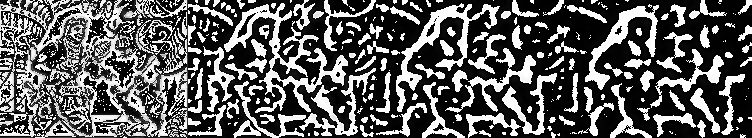
\includegraphics[scale=0.55]{bilder/firstDiv.png}
    	\caption{Differenz der Gaußfunktionen aus Abbildung \ref{fig:scaleSpace}. Die weißen Bereiche zeigen die Bereiche an, in denen Details verloren gehen.}

\label{fig:dogSample}
\end{figure}


Um die Differenz der Gaußfunktionen effizient zu berechnen, wird das Eingabebild mehrmals mit der Gaußfunktion gefaltet, um mehrere Skalierungen des Bildes zu erzeugen. Die einzelnen Skalierungen liegen immer um den Faktor $k$ auseinander.  Es werden jeweils von 2 Skalierungen, die im Skalenraum nebeneinander sind, die Differenz gebildet.
Sobald eine Oktave im Skalenraum durchlaufen ist, wird die Auflösung des Ursprungsbildes der Oktave halbiert. Dieses Bild bildet den Anfang der nächsten Oktave.
Dieser Vorgang wird in Abbildung \ref{fig:siftDog} dargestellt.

\begin{figure}[h]
    \centering
		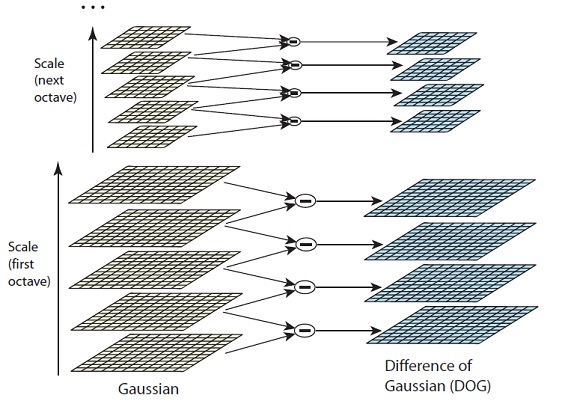
\includegraphics[scale=0.8]{bilder/sift-dog-idea.jpg}
    	\caption{Differenz der Gaußfunktionen für verschiedene Skalierungen und Oktaven (Abbildung aus \cite[S. 6]{Lowe2004}).}
\label{fig:siftDog}
\end{figure}

Um nun lokale Extrema im Scale Space zu finden, werden viele Beispielpunkte aus verschiedenen Skalierungen und Oktaven gewählt. Es werden drei Skalierungen pro Oktave betrachtet. Die Oktaven werden weitergeführt, bis die Bildauflösung zu gering ist.

Für jeden Punkt wird nun überprüft, ob er ein lokales Extremum ist. Dafür wird geprüft, ob der Punkt größer oder kleiner als alle seine Nachbarn in seiner eigenen Skalierung und in den Skalierungen darüber und darunter ist.

\begin{figure}[h]
    \centering
		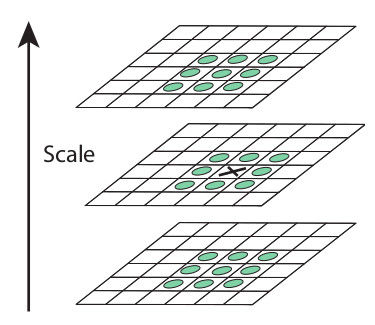
\includegraphics[scale=0.4]{bilder/sift_extrema.png}
    	\caption{Um ein Extremum zu sein, muss der mit X markierte Punkt größer oder kleiner sein als alle Nachbarn in anliegenden Scales (Abbildung aus\cite[S. 7]{Lowe2004}).}
\end{figure}

Viele der so gefunden Punkte sind nicht geeignet um stabile Merkmale zu sein:

Punkte mit zu geringem Kontrast (\ref{sec:kontrast}) sind nicht robust gegenüber Bildrauschen (\ref{sec:rauschen}). Durch den geringen Kontrast kann bereits leichtes Bildrauschen den Bereich stark verfälschen.
Deshalb werden von den potentiellen Merkmalen alle Punkte, deren Umgebung einen zu geringen Kontrast aufweist, entfernt.

Wie in \ref{sec:featureDetection} erwähnt, lassen sich Punkte entlang Kanten nicht gut an der Kante lokalisieren.

Der Gradient an Punkte, die an einer Kante liegen, ist in die Richtung der Kante sehr gering und in die Richtung entgegen der Kante sehr groß. Bei einer Ecke hingegen sind die Gradienten in alle Richtungen groß.
Für den Punkt wird die Richtung mit dem größten Gradienten gesucht und die Richtung rechtwinkling zu dieser. Ist das Verhältnis der Gradienten in die beiden Richtungen groß, so liegt der Punkt an einer Kante.

Um Punkte entlang Kanten zu entfernen, wird die Krümmung an dem jeweiligen Punkt betrachtet. Als Krümmung wird in diesem Zusammenhang die Ableitung der Gradiente verstanden. Die Richtung, in die die Krümmung am stärksten ist, wird als Hauptkrümmung bezeichnet.
Eine Kante hat eine starke Krümmung rechtwinklig zur Kante. Jedoch ist die Krümmung in Richtung der Kante sehr klein. 
Es wird nun das Verhältnis der Hauptkrümmung und der Krümmung rechtwickling zur Hauptkrümmung betrachtet.
Bei einer Ecke sind beide Krümmungen groß, also der Quotient der beiden gering. Bei einer Kante ist nur die Hauptkrümmung groß. Dadurch ist auch der Quotient groß. 
Ist das Verhältnis der beiden Krümmungen zu groß, wird der Punkt nicht mehr weiter betrachtet.


Die übrig gebliebenen Punkte werden nun Orientierungen zugewiesen und verwendet, um Merkmale zu bilden.


Um einem Punkt eine Orientierung zuzuweisen, wird für eine Region um ihn die Richtung $\theta(x, y)$ und Größe $m(x, y)$ der Gradienten berechnet. Das $\sigma$ entspricht der Skalierung, in der der Punkt gefunden wurde.
\[
m(x, y) = \sqrt{(L(x + 1, y, \sigma) - L(x - 1, y, \sigma))^2 + (L(x, y + 1, \sigma) - L(x, y - 1, \sigma))^2}
\]

\[
\theta(x, y)) = \tanh^{-1}((L(x + 1, y, \sigma) - L(x - 1, y, \sigma)) / (L(x, y + 1, \sigma) - L(x, y - 1, \sigma)))
\]

Es wird nun ein Histogramm der Gradientenrichtungen gebildet. Dieses Histogramm hat 36 Klassen, die jeweils 10° abdecken. Bei jedem hinzugefügten Punkt aus der Region wird dieser mit dem Gewicht $m(x, y)$ und einer Gaußgewichtung um den Ursprungspunkt des Ausschnittes gewichtet.
Aus dem Histogramm können nun durch die Spitzen die Orientierung der Region abgelesen werden. Sollte eine weitere Spitze nicht kleiner als 80\% der größten Spitze sein, wird für diese auch ein Merkmal erstellt. So enstehen für Regionen mit mehren Hochpunkten im Richtungshistogramm auch mehrere Merkmale.

\subsubsection{Merkmalsbeschreibung}

Nachdem einem Bildausschnitt eine Skalierung und eine Orientierung zugeordnet wurde, wird in diesem Schritt eine vektorielle Darstellung von diesem Aussschnit erstellt.


Der Deskriptor wird für eine $16 \times 16$ Umgebung um den Punkt gebildet. Hierbei wird für jeden Pixel in der Umgebung die Richtung $\theta(x, y)$ und Stärke $m(x, y)$ des Gradienten berechnet. Die Richtung wird um die zuvor gefundene Rotation gedreht, damit eine Unabhängigkeit von der Rotation gegeben ist.

Die Gradienten werden mit einem Gaußfenster gewichtet und in $4 \times 4$ Regionen eingeteilt (siehe Abbildung \ref{fig:siftDesc}). In diesen Regionen werden die Gradienten einer von 8 Richtungen zugeordnet, der sie am nächsten sind. Damit bildet jede Region einen 8 dimensionalen Merkmalsvektor. Der enstehende Deskriptor für den Bildausschnitt ist somit $4 \times 4 \times 8$.



\begin{figure}[h]
    \centering
		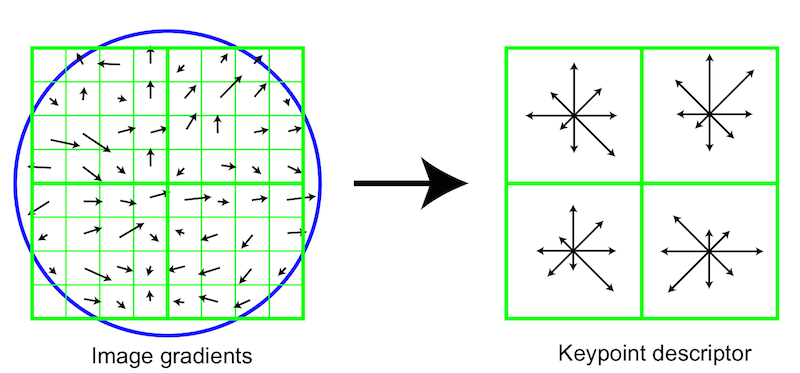
\includegraphics[scale=0.8]{bilder/sift_pic.png}
    	\caption{Umwandlung der Gradienten in den Descriptor für einen $8 \times 8$ Bildausschnitt. SIFT benutzt einen $16 \times 16$ Ausschnitt, aus dem ein $4 \times 4$ Descriptor erstellt wird.  Der blaue Kreis stellt die Gaußgewichtung dar (Abbildung aus\cite[S. 15]{Lowe2004}).}
 \label{fig:siftDesc}
\end{figure}



\subsection{Speeded Up Robust Features (SURF)}
Das Folgende Kapitel basiert auf dem Paper ''SURF: Speeded Up Robust Features'' von Herbert Bay.
\footnote{\cite{Bay:2008:SRF:1370312.1370556}}

Das Verfahren ''Speeded Up Robust Features'' (SURF) wurde von Herbert Bay 2006 vorgestellt. SURF ist ein Verfahren, das sowohl Merkmale findet, als auch Deskriptoren für diese bildet.
SURF versucht durch einige Approximationen schneller als SIFT zu sein ohne große Verluste in der Genauigkeit zu haben.

Für schnelle Berechnung von rechteckigen Filtern werden Integralbilder verwendet. Diese ermöglichen eine sehr schnelle Berechnung von Pixelsummen in einem rechteckigen Bildbereich.
In einem Integralbild ist jeder Pixelwert die Summe aller Pixel in einem Rechteck zwischen dem aktuellen Punkt und dem Bildursprung.

\[
I_i(x, y) = \sum_{i = 0}^{i < x} \sum_{j = 0}^{j < y} I(i, j)
\]

Nun kann die Summe der Pixelwerte eines Recktecks
 $R = \{ (x_1, y_1), (x_2, y_2), (x_3, y_3), (x_4, y_4)  \}$ mit nur vier Bildzugriffen berechnet werden.
\[
S(R) = I_i(x_1, y_1) + I_i(x_4, y_4) - I_i(x_2, y_2) - I_i(x_3, y_3)
\]



\subsubsection{Merkmalserkennung}

SURF nutzt die Determinante der Hesse-Matrix um Keypoints zu finden. Die Hesse-Matrix ist die zweite Ableitung einer mehrdimensionalen Funktion. Sie kann somit als ein Maß der Krümmung verstanden werden.
Es wird, ähnlich zu SIFT, in verschiedenen Skalierungen nach Maxima von $det(\mathcal{H}(x, y, \sigma))$ gesucht. Dabei ist die Hesse Matrix $\mathcal{H}(x, y, \sigma)$ für das Bild $I(x, y)$ und die Skalierung $\sigma$ definiert als:

\[
\mathcal{H}(x, y, \sigma) = 
\begin{bmatrix}
L_{xx}(x, \sigma) & L_{xy}(x, \sigma) \\
L_{xy}(x, \sigma) & L_{yy}(x, \sigma)
\end{bmatrix}
\]

Wobei $L_{xx}(x, y, \sigma)$ die Faltung von der zweifachen nach x abgeleiteten Gaußfunktion mit dem Bildpunkt ist. Das gleiche gilt für $L_{xy}(x, y, \sigma)$ und $L_{yy}(x, y, \sigma)$ in die entsprechenden Richtungen.

Um die Determinante schnell berechnen zu können, werden die partiellen Gaußableitungen mit rechteckigen Filtern approximiert. Diese seien im Folgenden $D_{xx}$, $D_{xy}$ und $D_{xy}$. Für die kleinste Skalierung $\sigma = 1.2$ wird ein $9x9$ Filter verwendet (siehe Abbildung \ref{fig:surfBox}).

SURF approximiert die Determinante mit 

\[
det(\mathcal{H}_{approx}(x, y, \sigma)) = D_{xx}D_{yy} - (0.9 D_{xy})^2
\]

In SIFT werden Gaußfilter mehrfach auf ein Bild angewandt, um höhere Skalierungen zu erhalten.
Der gleiche Effekt kann durch eine Erhöhung der Größe des Gaußfilters erreicht werden. Durch Integralbilder lässt sich die Filtergröße erhöhen, ohne mehr Berechnungen zu machen.
So nutzt SURF für die erste Oktave Filter der Größe $9x9, 15x15, 21x21, 27x27$. Der Abstand zwischen den Filtergrößen wird jede Oktave verdoppelt.


\begin{figure}[h]
    \centering
		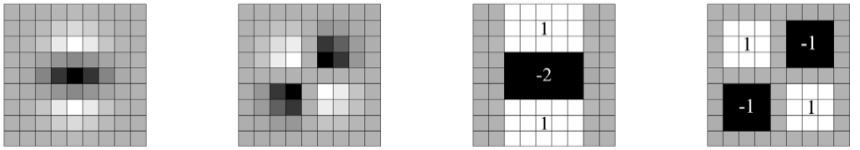
\includegraphics[scale=0.4]{bilder/surfBoxFilter.png}
    	\caption{Die Gaußfilter für die y und xy Richtung sowie deren Approximationen (Abbildung aus \cite{Bay:2008:SRF:1370312.1370556}).}
\label{fig:surfBox}
\end{figure} 


Um nun Keypoints in den verschiedenen Skalierungen zu finden, wird wie in SIFT geprüft, ob $det(\mathcal{H}(x, y, \sigma))$ an einem  Punkt in einer $3x3x3$ Nachbarschaft das Maximum ist.



\subsubsection{Merkmalsbeschreibung}

Der erste Schritt zur Erstellung des Deskriptors ist, dem Punkt eine Orientierung zuzuordnen. Sei $s$ im folgenden die Skalierung, in dem der Keypoint gefunden wurde.

Um dem Punkt eine Orientierung zuzuweisen, werden Haar Merkmale (siehe \ref{sec:haar}) verwendet. 
Es werden jeweils die Haar Merkmale in x und y Richtung bestimmt. Hierfür werden die Regionen in Abbildung \ref{fig:haar} mit einer Seitenlänge von $4s$ verwendet. Durch die Verwendung von Integralbildern sind diese Berechnungen sehr effizient.


Mit der gefunden Orientierung wird ein $20s$ großes Quadrat um den Punkt gelegt, welches um die Orientierung gedreht wird.
Dieses Quadrat wird in $4 \times 4$ Regionen unterteilt. In diesen Regionen wird ein 4-dimensionaler Merkmalsvektor bestimmt. Dieser Vektor besteht aus den Summen der horizontalen und vertikalen Haar Merkmale $dx$ und $dy$ in der Region(siehe Abbildung \ref{fig:surfFeature}). 
Die Größe der Regionen wird als $2s$ gewählt. Der Vektor ist definiert als: 

\begin{figure}[h]
    \centering
		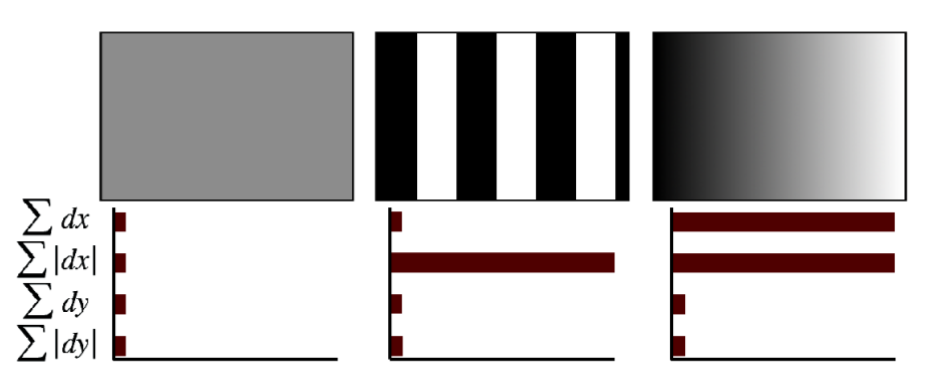
\includegraphics[scale=0.4]{bilder/surfFeature.png}
    	\caption{Die Größe der jeweiligen Merkmale für die gezeigten Bildausschnitte. Die einzelnen Komponenten des Vektors beschreiben die Strukturen der Intensität (Abbildung aus \cite{Bay:2008:SRF:1370312.1370556}).}
\label{fig:surfFeature}
\end{figure} 


\[
v = (\sum dx, \sum  |dx|, \sum dy, \sum |dy|)
\]

Aus den $4 \times 4$ Vektoren der einzelnen Regionen wird der Gesamtdeskriptor für das Merkmal gebildet.
Dadurch ensteht für jedes Merkmal ein 64-dimensionaler Vektor, der dieses Merkmal beschreibt.

\subsection{Oriented FAST and Rotated BRIEF (ORB)}
Das folgende Kapitel basiert auf dem von Ethan Ruble veröffentlichtem Paper ''ORB: an efficient alternative to SIFT or SURF'' \footnote{\cite{Rublee:2011:OEA:2355573.2356268,}}.

ORB wurde 2011 von Ethan Ruble als eine alternative zu SIFT und SURF vorgestellt, die deutlich schneller sein und dabei jedoch eine vergleichbar gute Perfomance haben sollte.
ORB kombiniert mehrere bestehende Verfahren und erweitert diese, um mit Rotation umgehen zu können. So wird FAST und ein Harris-Corner Detector \footnote{\cite{Harris88alvey}} verwendet, um Keypoints zu finden. Zudem werden die ''Binary Robust Independent
Elementary Features'' (BRIEF) \footnote{\cite{Calonder:2010:BBR:1888089.1888148,}} für die Merkmalsbeschreibung verwendent und so erweitert, dass sie mit der Rotation von Bildausschnitten umgehen können.

\subsubsection{Merkmalserkennung}

Um eine erste Auswahl an möglichen Keypoints zu erhalten wird FAST (siehe \ref{sec:fast}) verwendet.


FAST findet jedoch auch viele Punkte, die an einer Kante liegen und keine Ecke sind. Um diese herauszufiltern, wird der Harris-Corner Detector verwendet. Dieser gibt für einen Punkt ein Maß an, wie sehr dieser Punkt eine Ecke ist \footnote{\cite{Harris88alvey}}.


Für alle von FAST gefundenen Punkte wird der Harris Wert berechnet.
Um eine gewisse Anzahl $N$ an Punkten zu finden, wird  eine Schwelle $t$ zuerst so klein gewählt, dass mehr als $N$ Punkte über dieser liegen. Diese Punkte werden dann nach ihrem Harris Wert geordnet und die $N$ größten ausgewählt.
Damit die Merkmale Skalierungsinvariant sind, wird dies für mehrer Skalierungen des Bildes durchgeführt.

Da die von FAST gefundenen Punkte keine Orientierung haben, wird jedem gefundenen Merkmal noch eine Orientierung zugewiesen.
Dafür wird der Intensitätsschwerpunkt genutzt. Dieser liegt bei einer Ecke versetzt vom Mittelpunkt des betrachteten Bildausschnitts.
Um den Intensitätsschwerpunkt zu finden, werden die Momente des Ausschnittes betrachtet.
Momente in der Bildverarbeitung sind gewichtetete Intensitäten der Pixel eines Bildes bzw. eines Bildausschnittes.
Der Moment des $p$ und $q$ Grades, mit $p, q \in \mathbb{R}$ ist definiert als:

\[
m_{pq} = \sum_{x, y} x^p y^q I(x, y)
\]

Aus den Momenten $m_{00}, m_{01}$ und $m_{10}$ lässt sich der Schwerpunkt bestimmen.

\[
C =  \bigg(\frac{m_{10}}{m_{00}} , \frac{m_{01}}{m_{00}}\bigg)
\]

Die Orientierung des Keypoints wird definiert als der Vektor vom Zentrum bis zum Intensitätsschwerpunkt (siehe Abbildung \ref{fig:centroid}).

\begin{figure}[h]

    \centering
		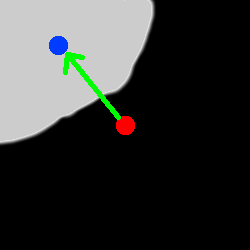
\includegraphics[scale=0.65]{bilder/centroid.png}
    	\caption{Der rote Punkt ist das Zentrum des Bildausschnitts und der blaue Punkt markiert den Intensitätsschwerpunkt. Der grüne Vektor zwischen den beiden bestimmt die Orientierung des Bildausschnitts.}
\label{fig:centroid}
\end{figure}


\[
\theta = \atantwo (m_{01}, m_{10})
\]

Diese Orientierung wird in $2\pi / 30$ große Abschnitte unterteilt.

\subsubsection{Merkmalsbeschreibung}

Um einen Deskriptor für ein gefundenes Merkmal zu bilden, wird ein $31 \times 31$ Bildausschnitt $p$ um den Keypoint betrachtet.
ORB benutzt eine um Rotation erweiterte Variante von BRIEF.
BRIEF erstellt einen binären Vektor aus einfachen Intensitätsvergleichen von zwei Bildpunkten. Hierfür wird der Bildausschnitt $p$ zuerst mit einem Gaußfilter geglättet.

Der binäre Test $\tau$ für den Bildausschnit $p$, wobei $p(x)$ die Intenstität an Bildpunkt x ist, ist definiert als:

\[
\tau(p; x, y) = 
\begin{cases}
1, & p(x) < p(y) \\
0, & p(x) \geq p(y)
\end{cases}
\]

Die Bitfolge der Testergebnisse ergibt sich aus:

\[
f_n(p) = \sum_{1 \leq i \leq n} 2^{i-1} \tau (p; x_i, y_i)
\]



Definiere die $2 \times n$ Matrix $S$ für alle n Vergleichspunkte $(x_i, y_i)$:

\[
S = \begin{pmatrix}
x_1 & \hdots & x_n \\
y_1 & \hdots & y_n 
\end{pmatrix}
\]

Für den Winkel $\theta$ des Bildausschnitts wird die Rotationsmatrix $R_\theta$ definiert, welche die Punkte in $S$ um $\theta$ dreht.

\[
S_\theta = R_\theta S
\]


\[
g_n(p, \theta) = f_n(p)|(x_i, y_i) \in S_\theta
\]


In der $31 \times 31$ Umgebung um den Keypoint gibt es eine hohe Anzahl an Bildpunkten, die miteinander verglichen werden könnten. Von all diesen Paaren $(x, y)$ sollen 256 ausgewählt werden.
Damit der Deskriptor möglichst diskriminierend ist, sollen Paare gewählt werden, die für eine große Menge an Bildausschnitten, auf denen sie ausgeführt werden, folgenden Eigenschaften haben:
\begin{itemize}

\item  Der Mittelwert des Testergebnisses liegt möglichst nah an $0.5$, also liefert der Test für verschiedene Bilder oft verschiedene Ergebnisse

\item Die Korrelation zwischen den gewählten Tests sollte möglichst gering sein, sodass jeder Test neue Informationen hinzubringt

\end{itemize}

Um die Testpaare zu lernen nutzt ORB ein Trainingsset von ca. 300000 Merkmalen aus dem PASCAL 2006 Bildersatz. Eine Auswahl der gelernet Testpaare ist in Abbildung \ref{fig:orbPairs} dargestellt.

\begin{figure}[h]

    \centering
		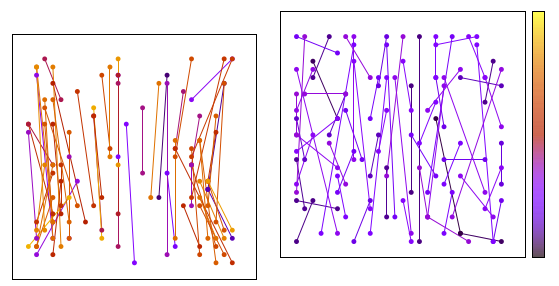
\includegraphics[scale=0.5]{bilder/orbPairs.png}
    	\caption{Darstellung einer Auswahl an Testpaaren. Die linke Seite zeigt Testpaare, die eine hohe Varianz besitzen. Die rechte Seite zeigt die Tests, nachdem der Trainingsschritt abgeschlossen wurde. Die Farben zeigen die maximale Korrelation eines Tests an. Schwarz und Lila stellen die geringste Korrelation dar. }
\label{fig:orbPairs}
\end{figure}

Es werden zuerst alle möglichen Testpaare für alle Keypoints berechnet und nach dem Abstand ihres Mittelwertes zu $0.5$ sortiert. 
Zunächst wird der Test, dessen Mittelwert am nächsten an $0.5$ dran ist, in die Ergebnismenge hinzugefügt.


Nun wird die sortierte Liste an Testpaaren durchgelaufen und ein Test zur Ergebnissmenge hinzugefügt wenn, seine Korrelation unter einem Schwellwert liegt. Ist das der Fall, wird der Test aus der sortierten Liste entfernt. Dies wird solange durchgeführt bis 256 Tests in der Ergebnismenge sind. 
Wird die Liste komplett durchlaufen und die Ergebnismenge ist kleiner als 256, wird der Schwellwert verringert und die Liste noch einmal neu durchlaufen.

Die so gefundenen 256 Testpaare bilden nun den ORB Deskriptor.